\documentclass[11pt]{article}

\usepackage{fullpage}
\usepackage{graphicx}
\usepackage{float}
\restylefloat{table}

\newcommand{\define}[2] {
  \textbf{Definition: #1}
  \begin{center} #2
\end{center}
}

\begin{document}

\section{Lecture 1: Introduction}

There is a diversity of methods currently used in Neuroscience:

\begin{enumerate}
\item Psychophysics
\item EEG/ERP
\item MEG
\item MRI/fMRI
\item Single neuron recordings and multiple neuron recordings
\end{enumerate}

We can also consider whether methods are invasive(directly interferers with neurons\cite{check}) or non-invasive. 

\subsection*{Psychophysics}
Psychophysics is a sub-discipline of psychology dealing with the relationship between physical stimuli and their perception. It is interested in measuring thresholds of perception, detection, discrimination. Measures illusions, reaction times, effects of training, group differences, effect of substance intake etc. It is non-invasive.  

\subsection*{Models}
A tool of neuroscience is mathmatical and computer models which are used to understand how the brain works. The aims are 

\begin{enumerate}
\item What? Description: unify data in a single framework
\item How? Understand mechanisms
\item Why? Interpretive model: Understand principles underlying functions
\item Make predictions - guide experiments and better data analysis
\end{enumerate}

\section{Lecture 2: Encoding}

\subsection{Neurons}
\define{Dendrites}{receive inputs from other cells}
\define{Axon}{transfers signal to other neurons}
\define{Synapse}{Contact between pre and post synaptic cell. Efficiency of transmission can vary over time.}
\define{Ion channels}{There are ion channels across the membrane, allowing ions to move in and out with selective permeability (mainly Na+ and K+, $Ca_2$ and Cl-)}

\subsubsection{Electrophysiological recordings}
There are two types: intracellular recordings where a sharp electrode is placed inside the neuron patch electrode, sealed to the membrane and is used to view the $Vm$. $Extracellular$ where the electrode is placed near a neuron to view action potentials often in Vivo(possible awake animal). Was common to observe one neuron at a time, now use of arrays of electrodes is beginning. 

\subsubsection{Describing neurons activity}
One of the aims of neuroscience is to describe the activity of a neuron and what it responds to. For example, we can observe a neuron where visual stimuli is changing orientation. We can measure spike sequence, number of spikes or rate $r$. The variability of this is large and thus needs to be averaged over many trials.

$p(t) = \sum lav(t - t_{i})$

$r = \frac{no.spikes}{T}$

\subsubsection{Modelling the average firing rate}

\define{Tuning curves}{You modify an aspect of the stimulus and measure the r<s> (spike count rate)}

V1 neurons: highly selective to the orientation of the stimulus (e.g bar) flashed in their receptive field. Bellshape tuning curves such as gaussian are common.

\begin{figure}[H]
\centering
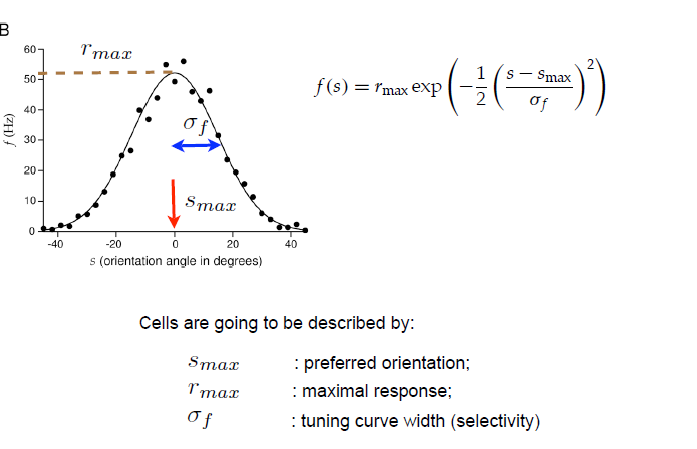
\includegraphics[width=90mm]{images/gaussian_tuning curve.png}
\caption{Gaussian tuning curve}
\label{old_house}
\end{figure}

\section{Lecture 3: Encoding}
\define{Encoding problem}{What is the relationship between stimuli in the world and the activity of the brain? $P(r|s)$}

Beyond simply just measuring the average spike count, we can use tools from probability theory: stochastic(random) processes. The spike count r on one trial is considered as a random variable. The probability of getting $n$ spikes is given by a probability distribution. For this we need the mean and variance. 

\subsection{Describing the variance of the spike count}
Measure the variance of the spike count for a number of repetitions with the same stimulus. Experiments show that the variance of the spike count is linearly related to the mean spike count. \textbf{Noise} of the model is often described as Poisson, or Gaussian with a variance proportional to the mean.

\subsection{Noise}
\subsubsection{Poisson distribution}
Is the probability of a spike count occurring in a fixed period of time, knowing average spike count f(s). The assumption is that the generation of each spike is independent of all other spikes. 

$P(n = k | s) = \frac{e^{-f(s)}f(s)^k}{k!}$

\subsubsection{Guassian noise model}
Another model that is commonly used to describe the variability ot the spike count is the Guassian noise model,. The activity can be described as:
$n = f(s) + n(s)$
$n(s) = N(0, o^2(s))$
To mimic Poisson process, we choose $o^2(s) = f(s)$

\subsubsection{Where does the Noise come from?}
Noise is commonly represented as a Poisson or Guassian distribution. Is the Poisson variability really noise? (unresolved, yet critical question)

\begin{enumerate}
\item Where could it come from?
\item Probably not in the sensory inputs
\item Probably not in the spike initiation mechanism
\item Probably not in the stochastic nature of opening/closing of ion channels
\item Probably not in the unreliable synapses
\end{enumerate} 

Variability could offer distinct advantages or emerge from deterministic Bayesian processes. 

\subsection{Encoding summary}
Spikes are the important signals in the brain. What is still debated is the code: number of spikes, exact spike timing, temporal relationship between neuron activities. 
Experimentalists have characterised the activity of neurons all over the brain and in particular in the sensory cortex, motor cortex etc, mainly in terms of $tuning curves$ and $response curves$. A variety of well specialised areas. Detailed wiring and mechanisms at the origins of these responses are widely known. 
The large variability is often well described by a Poisson or Gaussian model. 

\subsection{Questions}
Slide 5 "Experiments show that the variance of the spike count is linearly related to the mean spike count".
Humans are attempting to advance themselves by looking closer at the human brain. Effectively, to advance, we are learning to understand ourselves and how the brain works. This creates a problem - could computers and our technology be inhibited by our own brain? The best way for everyone to reach a better understanding is to all share knowledge. 

\section{Lecture 3: Overview of visual cortex}

\section{Lecture 4: Encoding}
I think most of the methods from this chapter are based on encoding?

Encoding could be used to give people hearing or vision again. Cochlear implants provide a sense of sound. 

\subsection{Decoding populations of neurons}
An estimation problem (detecting signal in noise)
Tools: Estimation theory, Bayesian inference, machine learning. 

\subsection{Optimal decoding}
Maximum likelihood
Maximum posteriori

\subsection{Simpler decoding strategies}

\subsubsection{Winner Take All}

\subsubsection{Population Vector}
Take all the vector orientations of the neurons preferred orientations. Sum these together and obtain a resultant vector. 

\section{Decision making}


\section{Lab notes}

\subsection{Lab 1}
Effectively for question 1 part b, we are modelling the activation spikes when the orientation changes.

\section{Coursera: Neurobiology}
Dendrites: Inputs in ESPS: Exitatory post-synaptic potential. If you receive enough of these it creates a spike action potential.
Axons: output of neuron

\section{Glossary}
\define{Psychophysics}{Investigates the relationship between physical stimuli and sensations and the perceptions they affect}
\define{Encoding:}{How does a stimulus cause a pattern of responses? P(response | stimulus)}
\define{Decoding:}{What do these responses tell us about the stimulus? How can we reconstruct what the brain is doing? $P(stimulus | response)$}
\define{Signal Detection Theory}{Ability to discern between information-bearing patterns and random patterns that distract from the information(noise)}

\end{document}